\documentclass[]{article}
\usepackage{lmodern}
\usepackage{amssymb,amsmath}
\usepackage{ifxetex,ifluatex}
\usepackage{fixltx2e} % provides \textsubscript
\ifnum 0\ifxetex 1\fi\ifluatex 1\fi=0 % if pdftex
  \usepackage[T1]{fontenc}
  \usepackage[utf8]{inputenc}
\else % if luatex or xelatex
  \ifxetex
    \usepackage{mathspec}
  \else
    \usepackage{fontspec}
  \fi
  \defaultfontfeatures{Ligatures=TeX,Scale=MatchLowercase}
\fi
% use upquote if available, for straight quotes in verbatim environments
\IfFileExists{upquote.sty}{\usepackage{upquote}}{}
% use microtype if available
\IfFileExists{microtype.sty}{%
\usepackage{microtype}
\UseMicrotypeSet[protrusion]{basicmath} % disable protrusion for tt fonts
}{}
\usepackage[margin=1in]{geometry}
\usepackage{hyperref}
\hypersetup{unicode=true,
            pdftitle={BIO8068 Data visualisation and management in ecology},
            pdfauthor={Roy Sanderson},
            pdfborder={0 0 0},
            breaklinks=true}
\urlstyle{same}  % don't use monospace font for urls
\usepackage{color}
\usepackage{fancyvrb}
\newcommand{\VerbBar}{|}
\newcommand{\VERB}{\Verb[commandchars=\\\{\}]}
\DefineVerbatimEnvironment{Highlighting}{Verbatim}{commandchars=\\\{\}}
% Add ',fontsize=\small' for more characters per line
\usepackage{framed}
\definecolor{shadecolor}{RGB}{248,248,248}
\newenvironment{Shaded}{\begin{snugshade}}{\end{snugshade}}
\newcommand{\KeywordTok}[1]{\textcolor[rgb]{0.13,0.29,0.53}{\textbf{#1}}}
\newcommand{\DataTypeTok}[1]{\textcolor[rgb]{0.13,0.29,0.53}{#1}}
\newcommand{\DecValTok}[1]{\textcolor[rgb]{0.00,0.00,0.81}{#1}}
\newcommand{\BaseNTok}[1]{\textcolor[rgb]{0.00,0.00,0.81}{#1}}
\newcommand{\FloatTok}[1]{\textcolor[rgb]{0.00,0.00,0.81}{#1}}
\newcommand{\ConstantTok}[1]{\textcolor[rgb]{0.00,0.00,0.00}{#1}}
\newcommand{\CharTok}[1]{\textcolor[rgb]{0.31,0.60,0.02}{#1}}
\newcommand{\SpecialCharTok}[1]{\textcolor[rgb]{0.00,0.00,0.00}{#1}}
\newcommand{\StringTok}[1]{\textcolor[rgb]{0.31,0.60,0.02}{#1}}
\newcommand{\VerbatimStringTok}[1]{\textcolor[rgb]{0.31,0.60,0.02}{#1}}
\newcommand{\SpecialStringTok}[1]{\textcolor[rgb]{0.31,0.60,0.02}{#1}}
\newcommand{\ImportTok}[1]{#1}
\newcommand{\CommentTok}[1]{\textcolor[rgb]{0.56,0.35,0.01}{\textit{#1}}}
\newcommand{\DocumentationTok}[1]{\textcolor[rgb]{0.56,0.35,0.01}{\textbf{\textit{#1}}}}
\newcommand{\AnnotationTok}[1]{\textcolor[rgb]{0.56,0.35,0.01}{\textbf{\textit{#1}}}}
\newcommand{\CommentVarTok}[1]{\textcolor[rgb]{0.56,0.35,0.01}{\textbf{\textit{#1}}}}
\newcommand{\OtherTok}[1]{\textcolor[rgb]{0.56,0.35,0.01}{#1}}
\newcommand{\FunctionTok}[1]{\textcolor[rgb]{0.00,0.00,0.00}{#1}}
\newcommand{\VariableTok}[1]{\textcolor[rgb]{0.00,0.00,0.00}{#1}}
\newcommand{\ControlFlowTok}[1]{\textcolor[rgb]{0.13,0.29,0.53}{\textbf{#1}}}
\newcommand{\OperatorTok}[1]{\textcolor[rgb]{0.81,0.36,0.00}{\textbf{#1}}}
\newcommand{\BuiltInTok}[1]{#1}
\newcommand{\ExtensionTok}[1]{#1}
\newcommand{\PreprocessorTok}[1]{\textcolor[rgb]{0.56,0.35,0.01}{\textit{#1}}}
\newcommand{\AttributeTok}[1]{\textcolor[rgb]{0.77,0.63,0.00}{#1}}
\newcommand{\RegionMarkerTok}[1]{#1}
\newcommand{\InformationTok}[1]{\textcolor[rgb]{0.56,0.35,0.01}{\textbf{\textit{#1}}}}
\newcommand{\WarningTok}[1]{\textcolor[rgb]{0.56,0.35,0.01}{\textbf{\textit{#1}}}}
\newcommand{\AlertTok}[1]{\textcolor[rgb]{0.94,0.16,0.16}{#1}}
\newcommand{\ErrorTok}[1]{\textcolor[rgb]{0.64,0.00,0.00}{\textbf{#1}}}
\newcommand{\NormalTok}[1]{#1}
\usepackage{graphicx,grffile}
\makeatletter
\def\maxwidth{\ifdim\Gin@nat@width>\linewidth\linewidth\else\Gin@nat@width\fi}
\def\maxheight{\ifdim\Gin@nat@height>\textheight\textheight\else\Gin@nat@height\fi}
\makeatother
% Scale images if necessary, so that they will not overflow the page
% margins by default, and it is still possible to overwrite the defaults
% using explicit options in \includegraphics[width, height, ...]{}
\setkeys{Gin}{width=\maxwidth,height=\maxheight,keepaspectratio}
\IfFileExists{parskip.sty}{%
\usepackage{parskip}
}{% else
\setlength{\parindent}{0pt}
\setlength{\parskip}{6pt plus 2pt minus 1pt}
}
\setlength{\emergencystretch}{3em}  % prevent overfull lines
\providecommand{\tightlist}{%
  \setlength{\itemsep}{0pt}\setlength{\parskip}{0pt}}
\setcounter{secnumdepth}{0}
% Redefines (sub)paragraphs to behave more like sections
\ifx\paragraph\undefined\else
\let\oldparagraph\paragraph
\renewcommand{\paragraph}[1]{\oldparagraph{#1}\mbox{}}
\fi
\ifx\subparagraph\undefined\else
\let\oldsubparagraph\subparagraph
\renewcommand{\subparagraph}[1]{\oldsubparagraph{#1}\mbox{}}
\fi

%%% Use protect on footnotes to avoid problems with footnotes in titles
\let\rmarkdownfootnote\footnote%
\def\footnote{\protect\rmarkdownfootnote}

%%% Change title format to be more compact
\usepackage{titling}

% Create subtitle command for use in maketitle
\newcommand{\subtitle}[1]{
  \posttitle{
    \begin{center}\large#1\end{center}
    }
}

\setlength{\droptitle}{-2em}

  \title{BIO8068 Data visualisation and management in ecology}
    \pretitle{\vspace{\droptitle}\centering\huge}
  \posttitle{\par}
  \subtitle{Further shiny development}
  \author{Roy Sanderson}
    \preauthor{\centering\large\emph}
  \postauthor{\par}
    \date{}
    \predate{}\postdate{}
  

\begin{document}
\maketitle

\subsection{1. Introduction}\label{introduction}

When designing and writing shiny applications it is easy to become
confused by the R code, as the code in the user-interface (\texttt{ui})
and \texttt{server} functions is difficult to debug. The simplest
approach is to compartmentalise different tasks, testing them in
standard R scripts, and either calling these at the start of the main
\texttt{app.R} code using the \texttt{source} function to setup various
initial parameters, creating functions than can be re-used later, or
integrating them into the \texttt{server} code once you know the
original R code is robust. Good coding practices will help you do this
effectively and well. Finally, you want others to be able to use your
shiny app, so you have to know how to publish it on the web. The main
aims of this practical are to:

\begin{itemize}
\tightlist
\item
  learn how to plan a shiny app, how to structure and test it
\item
  good coding practice, shiny reactive programming
\item
  publishing your app on the web
\end{itemize}

\subsection{2. Planning your shiny app}\label{planning-your-shiny-app}

Decide on who will be your users: how much technical skills will they
have, and what will they want to gain through using your shiny app? For
your assignment, assume that your end-users might be informed members of
the public, wanting to gain a more in-depth understanding of the
environment and ecology in Cumbria. Sketch out on paper what you would
like your shiny app to be able to show, what data (maps, graphs, tables)
do you want displayed. How might you want your user to interact with
your shiny app? Do you want the user to be presented with a single page,
that they can scroll down (much simpler to build), or separate tabs on a
dashboard (harder to code).

\subsection{3. Prototyping your shiny
app}\label{prototyping-your-shiny-app}

Spend some time thinking carefully about the user interface (UI) part of
your application. Ideally you want to design this and check that it
\emph{roughly} behaves as expected before you invest a lot of time on
the \texttt{server} code. A good place to start is the Shiny Gallery
where you can look at example interfaces, read their code, and even see
which lines of code are responding to different user-interactions
dynamically. You can find Shiny Gallery at
\url{https://shiny.rstudio.com/gallery/}

\begin{itemize}
\item
  Begin by looking at the the section marked \texttt{Start\ Simple}
  where you can learn about simple methods, particularly the ``iris
  dataset'' \url{https://shiny.rstudio.com/gallery/kmeans-example.html}
  scatterplot and ``Telephones by region''
  \url{https://shiny.rstudio.com/gallery/telephones-by-region.html}.
  \textbf{Note} Originally shiny apps had to be written with the
  \texttt{ui} and \texttt{server} in separate R files, but this is now
  optional and they can be both stored in a single \texttt{app.R} file.
\item
  The section entitled \texttt{Widgets} gives simple examples of how to
  use check boxes, drop-down lists, sliders, graphs, tables of data etc.
  Explore some of these, particularly those that you think might be
  useful to your app. \textbf{Exercise}: Copy the code of one or two
  widget examples and test them: this is the only real way of learning
  what they do.
\item
  Decide whether you want a long-style of website or a dashboard. An
  example long-style website is that of the USGS Biological Monitoring
  Station at Lake Erie
  \url{https://gallery.shinyapps.io/lake_erie_fisheries_stock_assessment_app/}.
  This is a single long page, with all the different graphical
  interfaces visible as you scroll down. Dashboards are more difficult
  to code, requiring the use of the \texttt{shinydashboard} add-on
  package \url{https://rstudio.github.io/shinydashboard/index.html}. As
  this is more complex, have a look at some of the examples before
  deciding whether to go down this route.
\end{itemize}

\subsection{4. Testing your prototype}\label{testing-your-prototype}

It is difficult to test a prototype user-interface without having all
the server components written already, which can be frustrating if you
want to focus on the user-interface design initially. The
\texttt{shinipsum} package comes with random plots, images, tables of
data etc. that you can use in an interface, without needing to worry
about the detail of the backend. The package is not available (yet) on
CRAN but can be installed from github:

\begin{Shaded}
\begin{Highlighting}[]
\CommentTok{# Note: installing shinipsum will also install lots of extra packages}
\NormalTok{remotes}\OperatorTok{::}\KeywordTok{install_github}\NormalTok{(}\StringTok{"Thinkr-open/shinipsum"}\NormalTok{)}
\end{Highlighting}
\end{Shaded}

You can then experiment by creating a very simple shiny app with some
random components. This one creates a user-interface with an image, a
ggplot, some printed output, a table, and some text. Obviously, the
values and contents are random.

\begin{Shaded}
\begin{Highlighting}[]
\KeywordTok{library}\NormalTok{(shiny)}
\KeywordTok{library}\NormalTok{(shinipsum)}
\KeywordTok{library}\NormalTok{(ggplot2)}
\NormalTok{ui <-}\StringTok{ }\KeywordTok{fluidPage}\NormalTok{(}
  \KeywordTok{h2}\NormalTok{(}\StringTok{"A Random Image"}\NormalTok{),}
  \KeywordTok{plotOutput}\NormalTok{(}\StringTok{"image"}\NormalTok{, }\DataTypeTok{height =} \StringTok{"300px"}\NormalTok{),}
  \KeywordTok{h2}\NormalTok{(}\StringTok{"A Random Plot"}\NormalTok{),}
  \KeywordTok{plotOutput}\NormalTok{(}\StringTok{"plot"}\NormalTok{),}
  \KeywordTok{h2}\NormalTok{(}\StringTok{"A Random Print"}\NormalTok{),}
  \KeywordTok{verbatimTextOutput}\NormalTok{(}\StringTok{"print"}\NormalTok{),}
  \KeywordTok{h2}\NormalTok{(}\StringTok{"A Random Table"}\NormalTok{),}
  \KeywordTok{tableOutput}\NormalTok{(}\StringTok{"table"}\NormalTok{),}
  \KeywordTok{h2}\NormalTok{(}\StringTok{"A Random Text"}\NormalTok{),}
  \KeywordTok{tableOutput}\NormalTok{(}\StringTok{"text"}\NormalTok{)}
\NormalTok{)}

\NormalTok{server <-}\StringTok{ }\ControlFlowTok{function}\NormalTok{(input, output, session) \{}
\NormalTok{  output}\OperatorTok{$}\NormalTok{image <-}\StringTok{ }\KeywordTok{renderImage}\NormalTok{(\{}
    \KeywordTok{random_image}\NormalTok{()}
\NormalTok{  \})}
\NormalTok{  output}\OperatorTok{$}\NormalTok{plot <-}\StringTok{ }\KeywordTok{renderPlot}\NormalTok{(\{}
    \KeywordTok{random_ggplot}\NormalTok{()}
\NormalTok{  \})}
\NormalTok{  output}\OperatorTok{$}\NormalTok{print <-}\StringTok{ }\KeywordTok{renderPrint}\NormalTok{(\{}
    \KeywordTok{random_print}\NormalTok{(}\StringTok{"model"}\NormalTok{)}
\NormalTok{  \})}
\NormalTok{  output}\OperatorTok{$}\NormalTok{table <-}\StringTok{ }\KeywordTok{renderTable}\NormalTok{(\{}
    \KeywordTok{random_table}\NormalTok{(}\DecValTok{10}\NormalTok{, }\DecValTok{5}\NormalTok{)}
\NormalTok{  \})}
\NormalTok{  output}\OperatorTok{$}\NormalTok{text <-}\StringTok{ }\KeywordTok{renderText}\NormalTok{(\{}
    \KeywordTok{random_text}\NormalTok{(}\DataTypeTok{nwords =} \DecValTok{50}\NormalTok{)}
\NormalTok{  \})}
\NormalTok{\}}
\KeywordTok{shinyApp}\NormalTok{(ui, server)}
\end{Highlighting}
\end{Shaded}

Try running the above code to produce your ``random'' user-interface.
The start to modify it to what you might want. e.g.~with a drop down
menu, or click boxes etc. The \texttt{shinipsum} does not allow you to
display a random \texttt{leaflet} map, but hopefully it will give you a
feel for how to assemble the user interface. The \texttt{shinipsum}
package also has options to display a random \texttt{ggplotly} graph and
random data-table display (requires \texttt{ggplotly} and \texttt{DT}
packages).

\subsection{5. Coding the server}\label{coding-the-server}

You will find it easiest to code different parts of the server backend
as separate R scripts, to check that they work correctly outside of
\texttt{shiny}, read any input data files etc. Sometimes you might be
able to use the \texttt{source} command near the top of your
\texttt{app.R} script, so that you can keep your main code uncluttered,
especially if you want to put your own user-written functions into
separate files. We did something similar in the first practical on
oystercatchers, where most of you put the \texttt{multiplot} function
into a separate R script called \texttt{multiplot.R} which you were able
to source from the start of your analysis, without cluttering up your
main code for the oystercatcher analysis.

\subsection{6. Good coding practice}\label{good-coding-practice}

It is worth using a consistent coding style, as it reduces errors and
makes it easier to spot mistakes. Here are a few hints:

\subsubsection{6.1 Object names}\label{object-names}

Moderate length names, that are clear and accurately describe what the
object contains or what it does are best. Variables using
\texttt{snake\_case} are usually easier to read than \texttt{CamelCase}.

\begin{verbatim}
# Good
total_sheep
population_size
soil_type
calc_rainfall  # This is obviously a function rather than a variable
plot_rivers    # A function, similar to the multiplot example

# Bad
tmp # I will admit guilt on this one!
TotSheep
PopulationNO
Rainfall_Amount
stagnohumic_gley_soil_per_ha
\end{verbatim}

\subsubsection{6.2 Comments}\label{comments}

Good comments are succinct but add to the clarity of the code. Use of
good variable and function names helps to make the code partially
self-documentating, but you will always need comments to remind both
yourself and others what you did. Imagine you will be readiing the code
in 6, 12 or 18 months time. Will you still be able to understand what it
says? I have sometimes looked at old code that I have written a year
earlier and puzzled about it. Also remember that if you end a comment
with \texttt{\#\#\#\#} or \texttt{-\/-\/-\/-} you automatically create a
table of contents to help you navigate your code. You can put long
comments on a series of separate lines, moderate ones on a single line,
or very short ones on the same line as code. Leave a space between the
\texttt{\#} symbol and the comment, so that you can easily use the
\textbf{CTRL-Shift-C} keyboard shortcut to comment and uncomment blocks
of text. Try to avoid comments more than 80 columns wide as they will
not print or display as easily. You can set RStudio to display an 80
column guideline.

\begin{verbatim}
# Good
# Read and clean raw soil data
# Function to display river data with vector input ####
# Next section reprocesses altitude data ----

# Next section of code derived from that published in Smith and Jones (2015)
# in Journal of Exciting Ecology, 23, 1-10.
grassland_type <- vegetation_community[nvc_type] # National Vegetation Class


# Bad
# Sort out the data
# Correct the errors earlier
# Tidy up the data
#Forgot to leave a space
# Next section of code derived from paper published that describes use of vegetation types in ecology and is relevant for this study 
grassland_type <- vegetation_community[nvc_type] # Assign grassland_type
\end{verbatim}

\paragraph{6.3 Spaces, assignments and
indentation}\label{spaces-assignments-and-indentation}

Good use of these relatively simple elements greatly improves
readibility.

\begin{verbatim}
# Assignment
rainfall <- 25 # Good
rainfall =  25 # Bad
rainfall=25    # Bad
rainfall<- 25  # Bad
rainfall  <-25 # Bad

# If you have assignments for related code, allign the operators
# Good
sheep_per_ha  <- 25
cattle_per_ha <- 8
pigs_per_ha   <- 2


# Bad
sheep_per_ha <- 25
cattle_per_ha <- 8
pigs_per_ha <- 2

# Indent with 2 spaces in general
# Good
if (y < 0 && debug) {
  message("Y is negative")
}

if (y == 0) {
  log(x)
} else {
  y ^ x
}

# Bad: no indentation
if (y < 0 && debug)
message("Y is negative")

# Bad: curly { brackets scattered across too many lines
if (y == 0)
{
  log(x)
} 
else
{
  y ^ x
}
\end{verbatim}

One exception to the 2 indent rule might be where you have a long
function with lots of function arguments that would run over multiple
lines, for example:

\begin{verbatim}
long_function_name <- function(a = "a long argument", 
                               b = "another argument",
                               c = "another long argument") {
  # As usual code is indented by two spaces.
}
\end{verbatim}

\subsection{7. Publishing shiny apps on the web for anyone to
use}\label{publishing-shiny-apps-on-the-web-for-anyone-to-use}

Currently you have `hosted' all your shiny apps on a `local' server,
that is on the PC on which you are developing your shiny application.
However, to allow anyone to use a shiny app you need to `publish' it on
an internet server. RStudio provides a `shiny server' application, which
you can run on your own internet-enabled server. However, this would
require you to manage the server, in particular to control security,
passwords etc. A simpler solution that also can be used when you don't
have a server, is to host your shiny app on the
\url{https://www.shinyapps.io/} website. You can sign-up for a free
account, and login with your github account. The free (Basic) allows a
maximum of 5 shiny applications, with 25 active hours. You can control
when to start or stop applications from within the shinyapps control
board.

\textbf{Note}: To learn how to use shinyapps.io I suggest you test it
out with a `dummy' shiny project (you can base it on the Old Faithful
geyser or one of the earlier simple shiny apps you have created).

Begin by logging into \url{https://www.shinyapps.io/} using your Github
username and password. The first time you sign in, shinyapps.io prompts
you to set up your account. Shinyapps.io uses the \textbf{account name}
as the domain name for all your apps. Account names must be between four
and 63 characters and can contain only letters, numbers, and dashes (-).
Account names may not begin with a number or a dash, and they can not
end with a dash (see RFC 952). Some account names may be reserved
already. So, if you use \textbf{davidsmith} as your account name, and
load up a shiny app called \texttt{rural-cumbria}, your web address will
be \texttt{https://davidsmith.shinyapps.io/rural-cumbria}. The text
\texttt{shinyapps.io} is present in the free account: you need to
subscribe to a paid service to have greater flexibility over the web
domain name.

\subsubsection{7.1 Deploying shiny apps}\label{deploying-shiny-apps}

Once you have setup your shinyapps.io account your are ready to deploy
your app. To do this you need to install the \texttt{rsconnect} package
and configure it to connect to your account:

\begin{Shaded}
\begin{Highlighting}[]
\KeywordTok{install.packages}\NormalTok{(}\StringTok{"rsconnect"}\NormalTok{)}
\KeywordTok{library}\NormalTok{(rsconnect)}
\end{Highlighting}
\end{Shaded}

Next, go to the shinyapps website, and after logging in via Github,
click on your user-name (top right) and the ``Tokens'' button:
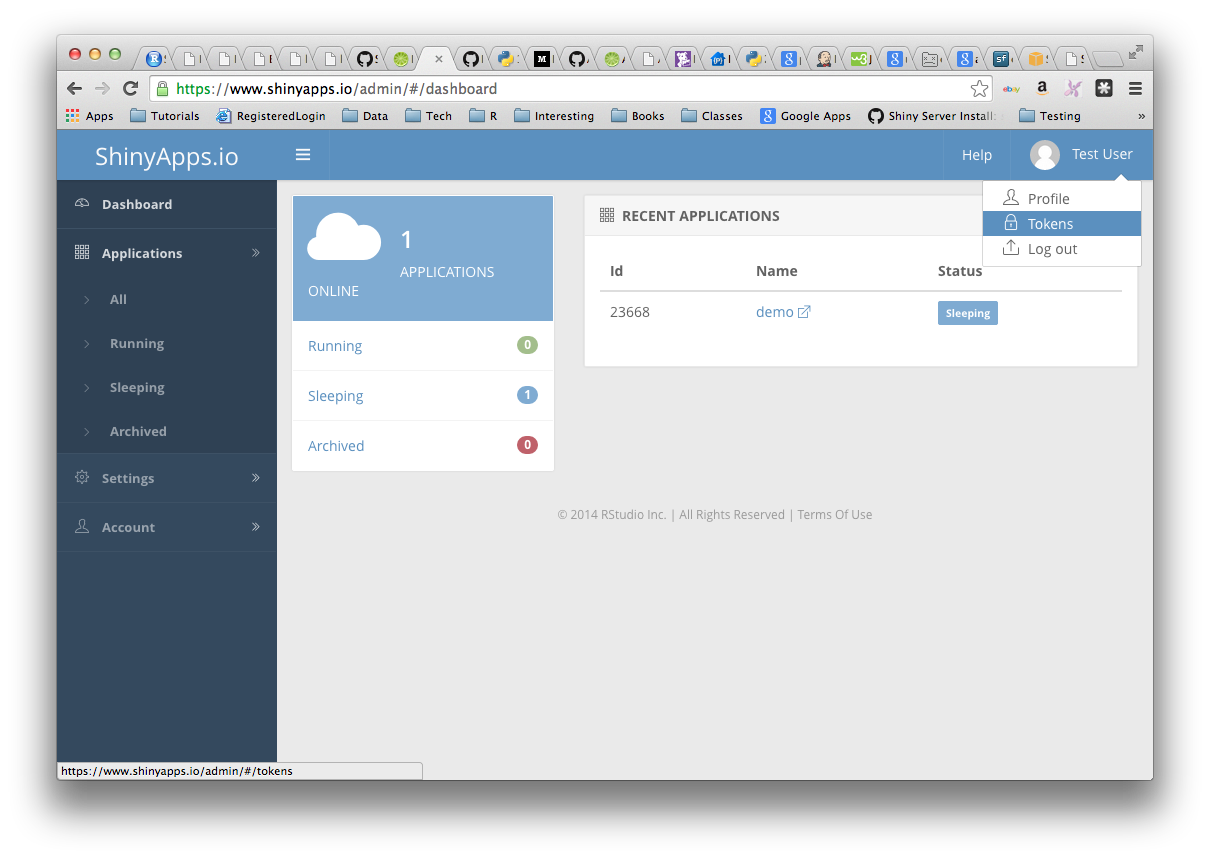
\includegraphics{figs/tokens.png} Click the Show button on the Token
page. A window will pop up that shows the full command to configure your
account using the appropriate parameters for the
rsconnect::setAccountInfo function. Copy this command to your clipboard,
and then paste it into the R \textbf{console} in the RStudio IDE and hit
Enter.

Now check that your shiny app runs: for this simple initial example I'm
assuming that you are using the Old Faithful geyser eruptions example.
(\textbf{Note}: on some machines I have sometimes encountered problems
deploying shiny apps from network drives, and if this proves to be a
problem, see below.) When you run the shiny app it will display in a
window by default:

\begin{figure}
\centering
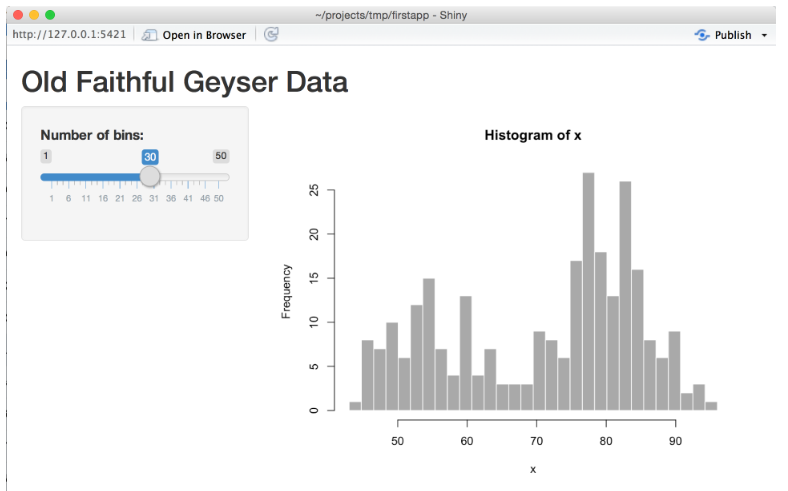
\includegraphics{figs/Old_Faithful.PNG}
\caption{}
\end{figure}

At the top-right is a button called ``publish'' and when you press this
your app should be deployed to shinyapps.io. A popup window will ask you
to confirm what is to be deployed. Note that if it is a large app, with
lots of packages to install, this may take a while, as the packages will
need to be installed on the remote deployed app. Alternatively, use the
\texttt{deployApp} command directly from the Console:

\begin{Shaded}
\begin{Highlighting}[]
\KeywordTok{library}\NormalTok{(rsconnect)}
\KeywordTok{deployApp}\NormalTok{()}
\end{Highlighting}
\end{Shaded}

and you should see something similar to the following, which takes about
3 to 4 minutes on my PC for the Old Faithful geyser example:

\begin{verbatim}
Preparing to deploy application...DONE
Uploading bundle for application: 787193...DONE
Deploying bundle: 1936830 for application: 787193 ...
Waiting for task: 595108460
  building: Fetching packages
  building: Installing packages
  building: Installing files
  building: Pushing image: 2027512
  deploying: Starting instances
  rollforward: Activating new instances
  success: Stopping old instances
Application successfully deployed to https://mep-ncl.shinyapps.io/OldFaithful/
Deployment completed: https://mep-ncl.shinyapps.io/OldFaithful/
\end{verbatim}

All being well, your shiny app will automatically open in a web-browser,
with an internet account.

\textbf{Possible problems}: the main problems I have encountered are
associated with the need for additional libraries and/or network drives.
Sometimes deployment requires additional libraries to be installed (e.g.
\texttt{RJSON}). Clicking the ``Publish'' button at the top right of
your shiny app seems more reliable at detecting this need. If when you
click the ``Publish'' button or issue \texttt{deployApp()} and nothing
happens (no messages on the screen) then the network drive might be
causing problems. You can resolve this issue by opening \emph{File
Manager} and copying your entire project file to
\texttt{C:\textbackslash{}TEMP\textbackslash{}\textless{}your\ user\ name\textgreater{}}
on your local machine. Then open RStudio again, and see if you can
deploy the app (you might need to confirm the tokens again).

\subsubsection{7.2 Working with the shinyapps.io
dashboard}\label{working-with-the-shinyapps.io-dashboard}

The shinyapps dashboard allows you to configure some aspects of your
apps. With a free account, you can only have 5 running applications, so
you may want to archive applications, or delete some with the
appropriate buttons. You can also change the amount of time before they
go from actively running into ``sleep'' mode. By default you get 25
hours of active CPU time per month for your apps with a free account,
which should be sufficient for this module. If you are concerned that
you might exhaust the limit (unlikely), reduce your ``sleep'' mode
time-out from the default of 15 minutes to 5 minutes.

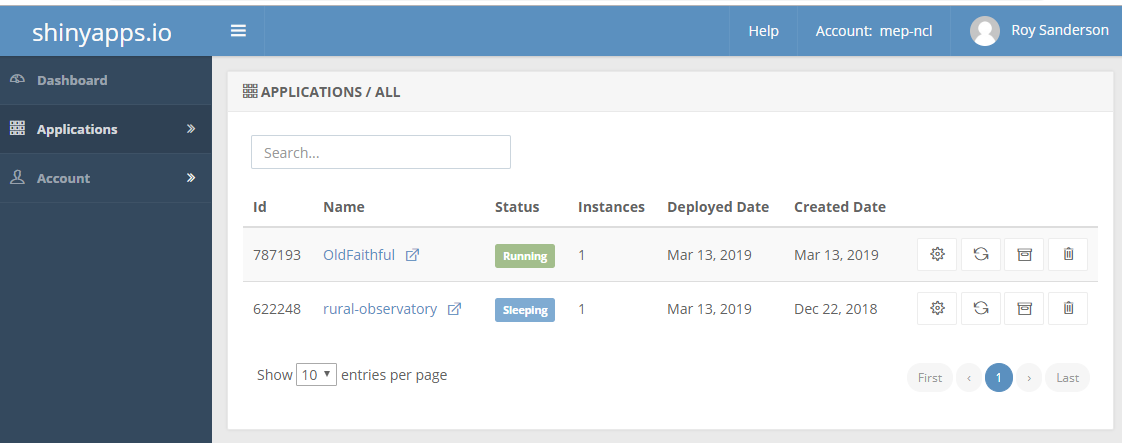
\includegraphics[width=0.5\linewidth]{figs/shinyapp_dashboard}


\end{document}
